\chapter{Приключения муравья Элиса}


\setlength{\epigraphwidth}{.67\textwidth}
\epigraph{Пойди к муравью, ленивец, посмотри на действия его, и будь мудрым.
}{--- Притчи Соломона 6:6-8} 

Муравьи, даже в одномерном мире, привлекают любителей головоломок и математиков.
Я приведу десяток головоломок (все они авторские, если не сказано обратное) про моего любимого муравья Элиса.
(См. рис. \ref{pic:alice1}.)
Каждая головоломка иллюстрирует какую-то математическую идею.

Начнём с классической муравьиной головоломки.

\begin{figure}[ht!]
\centering
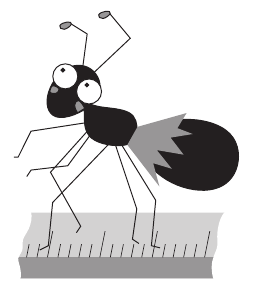
\includegraphics[scale=.5]{pics/alice1}
\caption{Муравей Элис, собственной персоной.}
\label{pic:alice1}
\end{figure}

\subsection*{Уже упал?}\label{Уже упал?}

На метровом стержне случайным образом расставлены двадцать пять муравьёв; наш Элис стоит тринадцатым с западного конца.
Каждый муравей повёрнут на восток или на запад с одинаковой вероятностью.
Муравьи начинают маршировать (туда, куда смотрят) со скоростью 1 см/сек;
при встрече, они меняют направление движения.
Сколько времени нужно подождать, чтобы быть точно уверенным в том, что Элис уже упал?

\subsection*{Элис на окружности}\label{Элис на окружности}

Теперь Элис один из 24 муравьёв, случайно расставленных на окружности метровой длины.
Каждый муравей случайно повёрнут по или против часовой стрелки и движется со скоростью 1 см/сек.
Как и раньше, при встрече муравьи разворачиваются.
Какова вероятность того, что через 100 секунд наш Элис окажется точно там, где начал?

\subsection*{Какой конец?}

Муравьи опять на стержне.
Какова вероятность того, что Элис упадёт с того конца, на который смотрел вначале?

\subsection*{Кто последний?}

Какова вероятность того, что Элис упадёт последним?

\subsection*{Число столкновений}

Во время всего процесса, каково ожидаемое (то есть среднее) число столкновений муравьёв?

\subsection*{Помятость Элиса}

Каково ожидаемое число столкновений у самого Элиса?

\subsection*{Страховой рейтинг Элиса}

Какова вероятность того, что у Элиса больше столкновений, чем у любого другого муравья?

\subsection*{Насморк}

Элис подхватил насморк, который мгновенно передаётся от муравья к муравью при столкновении.
Сколько муравьёв заразятся в среднем, прежде чем все упадут?

\subsection*{Элис посредине}

Проведём новый эксперимент.
Элис стоит точно посредине метрового стержня, 12 муравьёв расставлены случайным образом к западу от него, и ещё 12 к востоку.
Как и раньше, каждый муравей случайно повёрнут на восток или на запад, и каждый движется туда, куда смотрит, со скоростью 1 см/сек, меняя направление, при встрече лоб в лоб.
Однако на этот раз муравьи не падают;  
на концах стержня они разворачиваются и идут назад.
Через сто секунд муравьи застыли на месте.
На какое максимальное расстояние Элис сможет отойти от своего начального положения?

\subsection*{Новое место Элиса}

На стержне теперь только 24 муравья:
12 на западной половине смотрят на восток,
остальные на восточной половине смотрят на запад.
Элис --- пятый с западного конца.
Они движутся как обычно, разворачиваясь при столкновениях и падая с концов.
Что требуется знать об их начальной конфигурации, чтобы сказать, где очутится Элис через 63 секунды?
